\chapter{Governing equations}\label{sec:equations}

\def\Re{\mathrm{\bf Re}}
\def\Pr{\mathrm{\bf Pr}}
\def\Sc{\mathrm{\bf Sc}}
\def\Le{\mathrm{\bf Le}}
\def\Fr{\mathrm{\bf Fr}}
\def\Ro{\mathrm{\bf Ro}}
\def\Ma{\mathrm{\bf Ma}}
\def\Da{\mathrm{\bf Da}}

%%%%%%%%%%%%%%%%%%%%%%%%%%%%%%%%%%%%%%%%%%%%%%%%%%%%%%%%%%%%%%%%%%%%%%%%%%%%%%%%
%%%%%%%%%%%%%%%%%%%%%%%%%%%%%%%%%%%%%%%%%%%%%%%%%%%%%%%%%%%%%%%%%%%%%%%%%%%%%%%%
\section{Compressible formulation}

Let us consider first an ideal gas with one single species. The evolution equation for the energy is written in terms of the specific internal energy (sensible plus formation). Viscosity, thermal conductivity, diffusivity and the specific heat ratio can depend on the temperature. The governing equations are written as follows:
\begin{subequations}
    \begin{align}
        \partial_t \rho       =& -\partial_k (\rho u_k)                                       \\
        \partial_t (\rho u_i) =& -\partial_k (\rho u_i u_k )+\Re^{-1}\partial_k \tau_{ik}   \nonumber \\
        &  - \partial_i p +\Fr^{-1} \rho g_i\,b +\Ro^{-1}\rho\epsilon_{ijk} f_ku_j                         \\
        \partial_t (\rho e)   =& -\partial_k (\rho e u_k ) +\Re^{-1}\Pr^{-1} \partial_k \left(\lambda^{*}\partial_kT\right) \nonumber \\
        &-(\gamma_0-1)\Ma^2\,p\, \partial_k u_k  + (\gamma_0-1)\Ma^2\Re^{-1}\phi           \\
        \partial_t (\rho \zeta_i) =& -\partial_k (\rho \zeta_i u_k)-\Re^{-1}\Sc_i^{-1} \partial_k j_{ik}
    \end{align}
\end{subequations}
with
\begin{equation}
    \tau_{ij} \equiv \mu^*\left[\partial_j u_i +\partial_i u_j -(2/3)\, \partial_k u_k\,\delta_{ij}\right]\;,\qquad
    \phi      \equiv \tau_{ij} \partial_j u_i\;,\qquad
    j_{ik}    \equiv -(\rho D)_i^{*}\, \partial_k \zeta_i
\end{equation}
and
\begin{equation}
    \mu^{*} =  T^{n_\mu}\;,\qquad \lambda^{*} = T^{n_\kappa} \;,\qquad (\rho D)_i^{*}  =  T^{n_{D,i}}
\end{equation}
and
\begin{equation}
    p  = (\gamma_0 \Ma^2)^{-1}\rho T \;.
    \label{eq:state}
\end{equation}
The variables in these equations are normalized by the reference scales $\mathrm{L}_0$, $\mathrm{U}_0$, $\rho_0$ and $\mathrm{T}_0$, which represent a length, a velocity, a density, and a temperature, respectively. The pressure is normalized by $\rho_0U_0^2$. Thermal energy variables are normalized with $C_{p0}T_0$, where $C_{p0}$ is a reference specific heat capacity at constant pressure. $R_0$ is the specific gas constant of the gas under consideration. The dimensionless numbers are defined by
\begin{equation}
    \Re \equiv \frac{\rho_0 \mathrm{U}_0 \mathrm{L}_0}{\mu_0}\;, \qquad
    \Pr \equiv \frac{\mu_0}{(\lambda_0/C_{p0})}\;, \qquad
    \Sc_i \equiv \frac{\mu_0}{\rho_0 D_{i0}}\;,
\end{equation}
and
\begin{equation}
    \Ma  \equiv \frac{\mathrm{U}_0}{\sqrt{\gamma_0 R_0 \mathrm{T}_0}}\;, \qquad
    \gamma_0 \equiv \frac{C_{p0}}{C_{p0}-R_0}\;,
\end{equation}
and
\begin{equation}
    \Fr \equiv \frac{\mathrm{U}_0^2}{g\mathrm{L}_0} \qquad \Ro \equiv \frac{\mathrm{U}_0}{\mathrm{L}_0f} \;.
\end{equation}
Although $\gamma_0$ and $\Ma$ are the input parameters, the governing equations depend on $(\gamma_0\Ma^2)^{-1}$ and $(\gamma_0-1)\Ma^2$, which suggests to introduce the derived set of parameters
\begin{equation}
    (\gamma_0\Ma^2)^{-1}=\frac{R_0}{U^2_0/T_0}\;,\qquad (\gamma_0-1)\Ma^2 =\frac{U_0^2/T_0}{C_{p0}} \;,
\end{equation}
in the code implementation (names \texttt{RRATIO} and \texttt{CRATIO\_INV}, respectively). They can be interpreted as a normalized gas constant, and a normalized heat capacity. We also define $\gamma_0\Ma^2=U_0^2/(R_0T_0)$ as \texttt{RRATIO\_INV}, to save operations. The values of these parameters are defined in the procedure \texttt{Thermodynamics\_Initialize}.

%The body force is expressed in terms of the body force function $b^e(\rho,e,\zeta_j)$ and needs to be provided; the simplest case, $b^e=1$. 
The vectors $g_i$ and $f_i$ need to be provided and should be unitary, so that the magnitude of the term is completely determined by the corresponding nondimensional number. In this compressible case, the centrifugal term should probably be included; not yet studied.

\subsubsection{Multispecies}

Let us consider a mixture of $N$ species or constituents with mass fractions $Y_i$:
\begin{subequations}
    \begin{align}
        \partial_t \rho       =& -\partial_k (\rho u_k)                                                \\
        \partial_t (\rho u_i) =& -\partial_k (\rho u_i u_k )+\Re^{-1}\partial_k \tau_{ik}  \nonumber\\
        & -\partial_i p +\Fr^{-1} \rho g_i\,b +\Ro^{-1}\rho\epsilon_{ijk} f_ku_j                                     \\
        \partial_t (\rho e)   =& -\partial_k (\rho e u_k )+\Re^{-1}\Pr^{-1}\partial_k\color{red}{\left[(\lambda/C_p)^{*}\partial_kh\right]}\nonumber\\
        & \color{red}{+\Re^{-1}\Pr^{-1} \partial_k\left[\sum\left(\Le_i^{-1}(\rho D)_i^*
        -(\lambda/C_p)^*\right)h_i \partial_k  Y_i\right]}                                  \nonumber\\
        & -(\gamma_0-1)\Ma^2\,p\, \partial_k u_k  + (\gamma_0-1)\Ma^2\Re^{-1}\phi                 \\
        \partial_t (\rho \zeta_i)=& -\partial_k (\rho \zeta_i u_k) -\Re^{-1}\Sc_i^{-1} \partial_k j_{ik}
    \end{align}
\end{subequations}
and
\begin{equation}
    \mu^{*} = T^{n_\mu}\;,\qquad (\lambda/C_p)^{*} = T^{n_\kappa} \;,\qquad (\rho
    D)_i^{*} = T^{n_{D,i}}
\end{equation}
and
\begin{equation}
    \mathrm{\bf Sc}_i = \mathrm{\bf Le}_i \mathrm{\bf Pr}
\end{equation}
and
\begin{equation}
    Y_i = Y^e_i(\zeta_j)\;, \qquad \sum^N_1 Y_i=1
\end{equation}
\begin{equation}
    h = \sum^N_1 h_{i} Y_i \;,\qquad h_{i} = \Delta h^0_i + \int^{T}_{T_0}
    C_{pi}(T) dT\;,\qquad e = h - (\gamma_0-1)\Ma^2\frac{p}{\rho}
\end{equation}
\begin{equation}
    C_p = \sum^N_1 C_{pi}(T) Y_i\;,\qquad
    \gamma = \frac{C_p}{C_p-\frac{\gamma_0-1}{\gamma_0}R}
\end{equation}
and
\begin{equation}
    p = (\gamma_0 \mathrm{\bf Ma}^2)^{-1}\rho T R \;,\qquad
    R =\sum^N_1 R_iY_i\;.
\end{equation}
Each species has a specific heat capacity $C_{pi}$ and a specific gas constant $R_i=\mathcal{R}/W_i$,  where  $\mathcal{R}$ is the universal gas constant and $W_i$ the molar mass of the species. They are defined in the procedure \texttt{Thermodynamics\_Initialize}. They are nondimensionalized by the reference values $C_{p0}$ and $R_0=\mathcal{R}/W_0$, which are the values of one of the species. $R$ is the specific gas constant of the gas mixture nondimensionalized by $R_0$. $W=1/R$ is the mean molecular weight nondimensionalized by $W_0$, but we do not use this variable if the current implementation. 

Note that $\gamma_0$ is no longer an independent input parameter but is determined by the mixture in {Thermodynamics\_Initialize} as $\gamma_0=C_{p0}/(C_{p0}-R_0)$. As in the single species case, it proves convenient to introduce the derived parameters
\begin{equation}
    (\gamma_0\Ma^2)^{-1}=\frac{R_0}{U^2_0/T_0}\;,\qquad (\gamma_0-1)\Ma^2 =\frac{U_0^2/T_0}{C_{p0}} \;,
\end{equation}
in the code implementation (names \texttt{RRATIO} and \texttt{CRATIO\_INV}, respectively) and use 
\begin{equation}
    \tilde{R}\equiv (\gamma_0\Ma^2)^{-1}R=\sum_1^NY_i\,\tilde{R}_i\;,\qquad\tilde{R}_i\equiv (\gamma_0\Ma^2)^{-1}R_i
    \;,
\end{equation}
to save computation time and facilitate the consideration of a dimensional formulation in addition to the default nondimensional formulation here described (see below). 

Note that the specific heat ratio
\begin{equation}
    \gamma=\frac{C_p}{C_p-(\gamma_0-1)\Ma^2\tilde{R}}
\end{equation}
depends on the composition of the mixture and it is a derived (diagnostic) quantity.

\subsubsection{Dimensional Formulation}

In this case of a multi-species, a dimensional formulation can be considered by setting the input parameter \texttt{nondimensional} equal to \texttt{.false.} in the block \texttt{[Thermodynamics]} of the input file (by default, \texttt{tlab.ini}). The boundary and initial conditions defined in the input file should then be given in dimensional form. The code sets the parameters \texttt{RRATIO} and \texttt{CRATIO\_INV} equal to 1, and the equations above correspond to those of the dimensional formulation. 

The input parameters \texttt{Reynolds}, \texttt{Froude} and \texttt{Rossby} are then substituted by \texttt{Viscosity}, \texttt{Gravity} and \texttt{Coriolis}.

\subsubsection{On the difference between the species and the prognostic scalars}

The functions $Y_i^e(\rho,e,\zeta_j)$ need to be provided. We assume that $\sum_1^NY_i=1$ and use this relation to use $Y_N=1-\sum_1^N$ in the expressions above. For instance,
\begin{equation}
    \tilde{R}=\sum_1^{N-1}Y_i(\tilde{R}_i-\tilde{R}_N) \;.
\end{equation}
It is then clear that we do not need $Y_N$ as prognostic variable. More generally, the total number of species is $N$, need not be equal to the total number of scalars with an evolution equation. The former can be considered as part of the diagnostic variables and the latter as part of the prognostic variables. This includes the simplest possible case of $Y_i^e = \zeta_i$ for $i=1,\ldots,N-1$. 

Another case is equilibrium, e.g. Burke-Schumann approximation, where mass fraction of all species is related to the mixture fraction variable, $\zeta$.  In this case, the functions $Y_i^e(Z)$ are smoothed around $Z_s$ to reduce the strength of the discontinuity \citep{Higuera:1994}. The restriction of unity Lewis number the extra conditions $n_\mu=n_\kappa=n_D$ and $Sc=Pr$. These relationships are obtained by assuming equal diffusivity of all species and a single-step infinitely fast chemical reaction.  For further discussion on the formulation see \cite{Williams:1985}.

Another possible case is phase equilibrium (saturation adjustment), as considered for an mixture of air and water, where only the total water content is a prognostic variables and the partition into liquid and vapor is done assuming phase equilibrium. 

To reserve memory space for some of these diagnostic variables, the code implementation considers two global variables, namely, {\tt inb\_scal} and {\tt inb\_scal\_array}. The first one is the number of prognostic variables, and the latter is the number of prognostic and diagnostic variables. In principle, this should be specified through the variable {\tt imixture} in the input file. The average statistical data is calculated for all of them, prognostic and diagnostic variables.

\subsubsection{Reacting flows}

Add reaction terms to the scalar equations
\begin{equation}
    \partial_t (\rho \zeta_i)= -\partial_k (\rho \zeta_i u_k)
    - \mathrm{\bf Re}^{-1}\mathrm{\bf Sc}_i^{-1} \partial_k j_{ik} \color{red}{+\Da_i\,w_i}
\end{equation}
and $\Da_i$ are the Damk{\"o}hler numbers. A reaction mechanism needs to be given to obtain $w_i(\rho,e,\zeta_j)$.

%%%%%%%%%%%%%%%%%%%%%%%%%%%%%%%%%%%%%%%%%%%%%%%%%%%%%%%%%%%%%%%%%%%%%%%%%%%%%%%%
%%%%%%%%%%%%%%%%%%%%%%%%%%%%%%%%%%%%%%%%%%%%%%%%%%%%%%%%%%%%%%%%%%%%%%%%%%%%%%%%
\section{Incompressible formulation}

We need to solve a Poisson equation for the pressure. The thermodynamics is normalized differently.

\subsubsection{Anelastic formulation}

Dynamics and thermodynamics are still coupled by the background density and the buoyancy field. The evolution equations are:
\begin{subequations}
    \begin{align}
        0                 =& -\partial_k(\rho_\mathrm{bg}u_k)   & \\
        \partial_t  u_i   =& -\partial_k ( u_i u_k )-\rho_\mathrm{bg}^{-1}\partial_i p' &
        +\Re^{-1}\qquad\;\rho_\mathrm{bg}^{-1}\partial_k \left( \mu^{*} \partial_k u_i\right) & +\Fr^{-1}\, g_i\,b+\Ro^{-1}\,\epsilon_{ijk} f_k\,u_j  \\
        \partial_t\zeta_i =& -\partial_k (\zeta_i u_k) &
        + \Re^{-1}\Sc_i^{-1}\, \rho_\mathrm{bg}^{-1}\partial_k \left( \mu^{*}\partial_k\zeta_i\right) &+ \Da_i\,\rho_\mathrm{bg}^{-1}w_i
    \end{align}
\end{subequations}
where the buoyancy is
\begin{equation}
    b=\rho^{-1}(\rho_\mathrm{bg}-\rho)\approx\rho_\mathrm{bg}^{-1}(\rho_\mathrm{bg}-\rho) \;.
\end{equation}
The dynamic pressure $p'$ satisfies the following Poisson equation:
\begin{equation}
    \partial_i\partial_ip'=\partial_i\left[\rho_\mathrm{bg}\left(
    -\partial_k ( u_i u_k )+\Re^{-1}\rho_\mathrm{bg}^{-1}\partial_k \left( \mu^{*} \partial_k u_i\right) +\Fr^{-1}\, g_i\,b+\Ro^{-1}\,\epsilon_{ijk} f_k\,u_j
    \right)\right]\;.
\end{equation}
So far, only the case $\mu^*=1$ in the equations above has been implemented. The dynamic variables in these equations are  nondimensionalized by $\rho_0$, $U_0$ and $L_0$.

The thermodynamics is defined by the background profiles $\{\rho_\mathrm{bg},\, p_\mathrm{bg},\, T_\mathrm{bg},\, Y_\mathrm{bg}\}$, which are steady and satisfy the hydrostatic balance equation,
\begin{equation}
    \partial_2\,p_\mathrm{bg}=-\mathbf{H}^{-1}\, g_2\,\rho_\mathrm{bg}\;,\qquad p_\mathrm{bg}|_{x_2=x_{2,0}}=p_{\mathrm{bg},0}\;,
\end{equation}
and the thermal equation of state,
\begin{equation}
    p_\mathrm{bg}  = \rho_\mathrm{bg} R_\mathrm{bg} T_\mathrm{bg} \;.
\end{equation}
$\mathbf{g}$ is defined opposite to the gravitational acceleration (the problem is formulated in terms of the buoyancy). The background profile information in the input file {\tt tlab.ini}. The values $x_{2,0}$ and $p_\mathrm{bg,0}$ are provided through the background profile information for the pressure. 

The two equations above relate 4 thermodynamic variables, so we need two additional constraints. Typically, we impose the background profile of static energy (enthalpy plus potential energy) and the composition. In this case, the first scalar is the static energy
\begin{equation}
    \zeta_1 = h + \frac{\gamma_0-1}{\gamma_0}\mathbf{H}^{-1}(x_2-x_{2,0}) \;.
\end{equation}
The remaining scalars are the composition (e.g., total water specific humidity and liquid water specific humidity in the case of the airwater mixture). If there is only one species, then $R_\mathrm{bg}=1$ and we only need one additional constraint. 

The thermodynamic variables are nondimensionalized by $\rho_0$, $T_0$ and $R_0$, such that $p_0=\rho_0R_0T_0$. (Note the difference with the compressible formulation, where the pressure was nondimensionalized with $\rho_0U_0^2$.) The equations depend on the nondimensional parameter
\begin{equation}
    (\gamma_0-1)/\gamma_0 \;,
\end{equation}
a conversion factor between gas constants and heat capacities (thermal equation of state and caloric equation of state). We refer to it in the code as \texttt{GRATIO}. The default reference values are $p_0=10^5$~Pa and $T_0=298$~K, and are set in \texttt{Thermodynamics\_Initilize}. 

The nondimensional scale height is
\begin{equation}
    \mathbf{H} = \frac{R_0T_0}{gL_0} \;.
\end{equation}
This is a new thermodynamic parameter that appears in the anelastic formulation and needs to be provided in \texttt{tlab.ini}. 

A dimensional formulation can be considered by setting the parameter \texttt{nondimensional} equal to \texttt{.false.}, which sets \texttt{GRATIO} equal to 1

\subsubsection{Incompressible formulation}

Dynamics and thermodynamics are at most coupled by the buoyancy field, and thermodynamics is not necessary (but can still be used). With an appropriate form of the buoyancy function (see below), this formulation includes the Boussinesq limit. The evolution equations are :
\begin{subequations}
    \begin{align}
        0                   =& -\partial_k u_k                                          \\
        \partial_t  u_i     =& -\partial_k ( u_i u_k )  
        +\Re^{-1}\qquad\;\partial_k \left( \mu^{*} \partial_k u_i\right)  -\partial_i p&&
        +\Fr^{-1}\, g_i\,b +\Ro^{-1}\,\epsilon_{ijk} f_k\,u_j  \\
        \partial_t \zeta_i  =& -\partial_k (\zeta_i u_k)                    
        +\Re^{-1}\Sc_i^{-1}\, \partial_k \left( \mu^{*}\partial_k\zeta_i\right) &&+ \Da_i\,w_i
    \end{align}
\end{subequations}
So far, only the case $\mu^*=1$ in the equations above has been implemented.

Because of the decoupling between the momentum and the internal energy evolution equations, one of the scalar equations can correspond to the internal energy equation. Reaction or phase change processes, as well as radiation processes, can then be formulated as the appropriate source terms $\mathrm{\bf   Da}_\mathrm{L}w_\mathrm{L}$ and $\mathrm{\bf Da}_\mathrm{R}w_\mathrm{R}$, respectively, in the corresponding scalar equation. %Note that the physical meaning of the corresponding (generalized) Damk{\"o}hler numbers $\mathrm{\bf   Da}_\mathrm{L}$ and $\mathrm{\bf Da}_\mathrm{R}$ is a nondimensional heat parameter, and not a timescale ratio -- which is the correct meaning of the Damk{\"o}hler numbers appearing in the evolution equations for the components in a compressible mixture. We maintain this inconsistency, instead of introducing new symbols and variables, for code simplicity.

The formulation of the thermodynamics is the same as in the anelastic formulation.

\section{Particle formulation}

Lagrange formulation to describe the evolution of a set of particles.

To be done.

\section{Optional Phenomena}

\subsection{Body force}

In the incompressible case, $b(\mathbf{x},t)=b^e(\zeta_i(\mathbf{x},t),\mathbf{x},t)$ and the buoyancy function $b^e(\zeta_i,\mathbf{x},t)$ needs to be provided. The buoyancy function is assumed to be normalized by a reference buoyancy (acceleration) $b_0$ so that $\Fr=U_0^2/(b_0L_0)$. (Note that nondimensional numbers represent the relative magnitude of physical processes and thus they are positive semi-definite; the sign or direction associated with the process, if any, in indicated in the corresponding parameters.)

For the buoyancy function (see routine {\tt mappings/fi\_buoyancy}), the common expressions are a linear or bilinear relation to the scalar fields as
\begin{equation}
    b^e=\alpha_1\zeta_1+\alpha_2\zeta_2+\ldots+\alpha_\mathrm{\tt inb\_scal\_array+1} -b_\mathrm{ref}(x_2)\;,
\end{equation}
where the coefficients $\alpha_i$ need to be provided. A quadratic form
\begin{equation}
    b^e=-\frac{4\alpha_0}{\alpha_1^2}\zeta_1(\zeta_1-\alpha_1) -b_\mathrm{ref}(x_2)
\end{equation}
is also available, so that the maximum buoyancy $\alpha_0$ is achieved at
$\zeta_1=\alpha_1/2$.

The reference profile $b_\mathrm{ref}(x_2)$ is used to remove the hydrostatic balance to leading order and reduce the numerical error when calculating the pressure from the Poisson equation. (The exact form is not important because the Poisson equation provides the corresponding part of the hydrostatic balance.) To consider the background variation of density, there is also the class
\begin{equation}
    b(\mathbf{x},t)=(\zeta_1(\mathbf{x},t)-\langle \zeta_1\rangle)/\langle \zeta_1\rangle \;,
\end{equation}
where angle brackets indicate an average over the horizontal directions.



% Another option is a piece-wise linear function
% \begin{equation}
%     b^e=\frac{\alpha_2}{\alpha_3}\zeta_1+\\
%     \left(\frac{\alpha_1-\alpha_2}{1-\alpha_3}-\frac{\alpha_2}{\alpha_3}\right)
%     \alpha_4\ln\left[\exp\left(\frac{\zeta_1-\alpha_3}{\alpha_4}\right)+1\right] \;.
% \end{equation}
% The first linear branch of this function varies between $b^e=0$ at $\zeta_1=0$
% and $b^e=\alpha_2$ at $\zeta_1=\alpha_3$; the second linear branch varies
% between $b^e=\alpha_2$ at $\zeta_1=\alpha_3$ and $b^e=\alpha_1$ at
% $\zeta_1=1$. The first-order discontinuity at $\zeta_1=\alpha_3$ is smoothed
% over an interval $\alpha_4$ in the $\zeta_1$-space. This expression can be
% written as
% \begin{equation}
%     \begin{aligned}
%         &b^e=\beta_1\,\zeta_1+\beta_2\,(\ell-1)\;,
%         \qquad \beta_1=\frac{\alpha_1-\alpha_2}{1-\alpha_3}\;,\qquad
%         \beta_2=\frac{\alpha_3\alpha_1-\alpha_2}{1-\alpha_3}\;,
%         \\
%         &\ell=\frac{\alpha_4}{\alpha_3}\ln\left[\exp\left(\frac{\alpha_3-\zeta_1}{\alpha_4}\right)+1\right] \;,
%     \end{aligned}
% \end{equation}
% where the symbols $\beta_i$ relate to those used in Stevens (2002) according to $\beta_1\equiv\delta_\text{d}b$, $\beta_2\equiv g\beta_\ell q_{\ell\text{,max}}$, normalized with an appropriate buoyancy scale. ($\alpha_1\equiv\delta_\text{d}b-g\beta_\ell q_{\ell\text{,max}}$, $\alpha_3\equiv g\beta_\ell q_{\ell\text{,max}}/(\delta_\text{d}b-\delta_\text{m}b)$, and $\alpha_2\equiv\alpha_3\delta_\text{m}b$.) The piece-wise linear function reduces to a linear function when $\beta_2=0$.

% The last case is the piece-wise bilinear expression
% \begin{equation}
%     \begin{aligned}
%         &b^e=\beta_1\,\zeta_1+\beta_2\,(\ell-1) + \alpha_5\,\zeta_2\;,\\
%         &\ell=\frac{\alpha_4}{\alpha_3}\ln\left[\exp\left(\frac{\alpha_3-\zeta_1-\alpha_3\beta_6\,\zeta_2}{\alpha_4}\right)+1\right]
%         \;,\qquad \beta_6=\alpha_6\alpha_5/\beta_2\;,
%     \end{aligned}
% \end{equation}
% which reduces to the previous piece-wise linear in the case
% $\alpha_5=\alpha_6=0$. (The reason to express the buoyancy in terms of the
% parameter $\alpha_6$ instead of directly in terms of $\beta_6$ is that we also
% need $\alpha_6$ for the analysis of the source term of the buoyancy evolution
% equation.)

Note that the buoyancy field is {\it always} treated as a diagnostic variable and the average statistical data -- actually from the momentum source term $\Fr^{-1}b$ -- is calculated as an additional scalar field on top of {\tt   inb\_scal\_array} scalars (prognostic plus diagnostic). The only exception occurs when the buoyancy function is merely a linear relation because, in that case, the corresponding statistical information can be easily obtained from the corresponding scalar field.

\subsection{Coriolis force}

The current formulation corresponds to that of an Ekman layer along an $Ox_1x_3$ plane. The direction $Ox_2$ is defined along the angular velocity, so that $f_1=f_3=0$. The momentum equation reads 
\begin{subequations}
    \begin{align}
        \partial_t  u_1 =& -\partial_k ( u_1 u_k ) -\partial_1 p &
        +\Re^{-1}\,\partial_k  \left( \mu^{*} \partial_k u_1\right) &
        +\Fr^{-1}\, g_1\,b +\Ro^{-1}\,f_2\,(u_{3,g}-u_3) \\
        \partial_t  u_2 =& -\partial_k ( u_2 u_k ) -\partial_2 p &
        +\Re^{-1}\,\partial_k  \left( \mu^{*} \partial_k u_2\right) &
        +\Fr^{-1}\, g_2\,b \\
        \partial_t  u_3 =& -\partial_k ( u_3 u_k ) -\partial_3 p &
        +\Re^{-1}\,\partial_k  \left( \mu^{*} \partial_k u_3\right) &
        +\Fr^{-1}\, g_3\,b +\Ro^{-1}\,f_2\,(u_1-u_{1,g})
    \end{align}
\end{subequations}
The geostrophic velocity vector $(u_{1,g},\,u_{2,g},\,u_{3,g}) = (\cos\alpha,\,0,\,-\sin\alpha)$ is defined in terms of the input parameter $\alpha$ (rotation angle around $Ox_2$), to be provided.

\subsection{Radiation}

Formally, radiation heating or cooling can be considered in the equations above as an additional source term $\mathrm{\bf Da}_\mathrm{R}\,\omega_\mathrm{R}\,\delta_{i\beta}$ in the right-hand side of one of the evolution equations, where $\mathrm{\bf Da}_\mathrm{R}$ is the corresponding nondimensional heat parameter and the radiation function $\omega_\mathrm{R}(\zeta_j)$ is normalized by the corresponding (dimensional) heat parameter $Q$. 

Practically, the implementation is completely embedded in the routine {\tt mappings/radiation} and uses data provided in the block \texttt{[Infrared]} or \texttt{[Visible]} (i.e., assumes $\mathrm{\bf Da}_\mathrm{R}=1$ and all coefficients enter in the definition of $\omega_\mathrm{R}$). 

In a one-dimensional model, the source term is expressed in terms of upward and downward fluxes according to
\begin{equation}
    \omega_\mathrm{R}=-\partial_z(F_\uparrow -F_\downarrow) \;.
\end{equation}
($F_\downarrow$ is defined positive going downwards.) The fluxes are obtained from the radiative transfer problem
\begin{equation}
    \bar{\mu}\, \partial_\tau F+F = B\;,\qquad F|_{\tau=0}=F_0 \;,
\end{equation}
where $\tau$ is the optical depth, $\bar{\mu}$ is a mean direction parameter and
\begin{equation}\label{equ:sb}
    B\equiv \sigma T^4
\end{equation}
is an emission function. Written in spatial coordinates using the change of variables $\mathrm{d}\tau = a\,\mathrm{d}s$, we obtain
\begin{equation}\label{equ:rte}
    \partial_s F+(a/\bar{\mu}) F = (a/\bar{\mu}) B\;,\qquad F|_{s=0}=F_0 \;,
\end{equation}
where $s$ is the distance and 
\begin{equation}
    a = \kappa_1 \rho \zeta_1 + \kappa_2 \rho \zeta_2 + \ldots
\end{equation}
is the absorption coefficient, the constants $\kappa_i$ being the corresponding mass absorption coefficients. The source term is then given by
\begin{equation}
    \omega_\mathrm{R}=(a/\bar{\mu}) (F_\uparrow +F_\downarrow) - 2(a/\bar{\mu}) B \;.
\end{equation}
(Note the change of variables $s=z_\mathrm{max}-z$ in the downward flux equation.) The mean direction is $\bar{\mu}\in[1/\sqrt{3},1/\sqrt{2}]$; we use the mean value over that interval. The solution to the radiative transfer problem yields
\begin{subequations}\label{rad:flux}
    \begin{align}
        F_\uparrow &= e^{-\tau(z_\mathrm{min},z)/\bar{\mu}}\left[ F_{\uparrow,z_\mathrm{min}} + \int_{z_\mathrm{min}}^z (a/\bar{\mu}) B e^{\tau(z_\mathrm{min},z')/\bar{\mu}}\mathrm{d}z'\right]\notag \\
        &= F_{\uparrow,z_\mathrm{min}}e^{-\tau(z_\mathrm{min},z)/\bar{\mu}}+ \int_{z_\mathrm{min}}^z (a/\bar{\mu}) B e^{-\tau(z',z)/\bar{\mu}}\mathrm{d}z' \;,\\
        F_\downarrow &= e^{-\tau(z,z_\mathrm{max})/\bar{\mu}}\left[ F_{\downarrow,z_\mathrm{max}} + \int_z^{z_\mathrm{max}} (a/\bar{\mu}) B e^{\tau(z',z_\mathrm{max})/\bar{\mu}}\mathrm{d}z'\right]\notag \\
        &=F_{\downarrow,z_\mathrm{max}}e^{-\tau(z,z_\mathrm{max})/\bar{\mu}} + \int_z^{z_\mathrm{max}} (a/\bar{\mu}) B e^{-\tau(z,z')/\bar{\mu}}\mathrm{d}z'\;,
    \end{align}
\end{subequations}
where the optical-depth function is defined as
\begin{equation}
    \tau(z_1, z_2) \equiv \int_{z_1}^{z_2}a(z')\mathrm{d} z'
\end{equation}
and we have used the relationship
\begin{equation}
    \tau(z_1, z_2) = \tau(z_1, z') + \tau(z', z_2)\;,\qquad z_1\le z'\le z_2 \;.
\end{equation}

Apart from the 2 implementations indicated in (\ref{equ:radflux}), we also consider the incremental formulation
\begin{subequations}\label{equ:radflux}
    \begin{align}
        &F_\uparrow(z_{i+1}) = e^{-\tau(z_i,z_{i+1})/\bar{\mu}}\left[ F_\uparrow(z_i) + \int_{z_i}^{z_{i+1}} (a/\bar{\mu}) B e^{\tau(z_i,z')/\bar{\mu}}\mathrm{d}z'\right]\notag  \;,\\
        &F_\downarrow(z_i) = e^{-\tau(z_i,z_{i+1})/\bar{\mu}}\left[ F_\downarrow(z_{i+1}) + \int_{z_i}^{z_{i+1}} (a/\bar{\mu}) B e^{\tau(z',z_{i+1})/\bar{\mu}}\mathrm{d}z'\right]\notag  \;,\\
    \end{align}
\end{subequations}
where $\{z_i\}_{i=1}^N$ is the set of grid points in which the interval $[z_\mathrm{min}, z_\mathrm{max}]$ is discretized. Note that we can write
\begin{equation}
    e^{-\tau(z_i,z_j)/\bar{\mu}}=\prod_{k=i+1}^{j}I_k\;,\qquad 
    I_k\equiv\left\{
    \begin{array}{ll}
        1 & k=1\;,\\
        e^{-\tau(z_{k-1},z_k)/\bar{\mu}} & k=2,\ldots N \;.
    \end{array}
    \right.
\end{equation}
Hence, we only need to compute and save $\{I_k\}_{k=1}^N$ and we can calculate any of the decay terms as necessary.

\subsubsection{Gray models}

We neglect the dependence on frequency in equation~(\ref{equ:rte}), or interpret it as an average equation over the frequency space.

One model that is implemented in the code sets the emission function to zero and consider only the liquid water. The input parameters are $F_{\downarrow,z_\mathrm{max}}$, $\kappa_\mathrm{l}$ and $F_{\uparrow,z_\mathrm{min}}$.

A second model considers liquid water and vapor and calculates $F_{\uparrow,z_\mathrm{min}}$ from the surface energy balance equation
\begin{equation}
    F_{\uparrow,z_\mathrm{min}} = \epsilon B(T|_{z_\mathrm{min}})+(1-\epsilon)F_\downarrow|_{z_\mathrm{min}} \;.
\end{equation}
The input parameters are $F_{\downarrow,z_\mathrm{max}}$, $\kappa_\mathrm{l}$, $\kappa_\mathrm{v}$ and the surface emissivity $\epsilon\in[0,1]$. Note that we need to solve first the problem for the downward flux to obtain its value at $z=z_\mathrm{min}$, use this equation to obtain the boundary condition for the upward flux, and then solve the problem for the upward flux.

\subsubsection{Band Models}

We partly retain the frequency dependence by considering frequency bands where the absorption coefficient is constant. We solve problem~(\ref{equ:rte}) separately for different bands:
\begin{equation}
    \partial_s F_\mathrm{b}+(a_\mathrm{b}/\bar{\mu}) F_\mathrm{b} = (a_\mathrm{b}/\bar{\mu}) B_\mathrm{b}\;,\qquad F_\mathrm{b}|_{s=0}=F_{\mathrm{b},0} \;,
\end{equation}
where the subscript $\mathrm{b}$ indicates band, 
\begin{equation}
    F_\mathrm{b}\equiv\int_{\nu_1}^{\nu_2}F_\nu\mathrm{d} \nu\;,
\end{equation}
the absorption coefficient of the band is
\begin{equation}
    a_\mathrm{b} = \kappa_{\mathrm{b},1} \rho \zeta_1 + \kappa_{\mathrm{b},2} \rho \zeta_2 + \ldots \;,
\end{equation}
and 
\begin{equation}
    B_\mathrm{b}(\nu_1,\nu_2,T)\equiv\int_{\nu_1}^{\nu_2}B_\nu(\nu,T)\mathrm{d} \nu\;,
\end{equation}
where the Planck function 
\begin{equation}
    B_\nu(\nu,T)\equiv c_{1L}\nu^3\frac{1}{\exp(c_2\nu/T)-1}\;,\qquad c_{1L}\equiv 2\pi hc^2\;,\qquad c_2\equiv hc/\kappa_B \;,
\end{equation}
is expressed in terms of the wavenumber $\nu$ (inverse of wavelength) and it is normalized such that
\begin{equation}
    \int_0^\infty B_\nu(\nu,T)\mathrm{d}\nu = B(T)\;,
\end{equation}
$B(T)\equiv\sigma T^4$ having been defined in~(\ref{equ:sb}). The integral of the Planck function over a finite interval of frequencies can be written as
\begin{equation}
    B_\mathrm{b}(\nu_1,\nu_2,T)=\beta_\mathrm{b}(T)B(T) \;,\qquad
    \beta_\mathrm{b}(T)\equiv\frac{15}{\pi^4}\int_{x_1(T)}^{x_2(T)}\frac{x^3}{e^x-1}\mathrm{d}x \;,
\end{equation}
and the limits of integration are $x_i(t)\equiv c_2\nu_i/T$. We assume that the union of all bands fills all the frequency space, so that
\begin{equation}
    \sum_\mathrm{b} \beta_\mathrm{b} =1\;.
\end{equation}
For a given band $(\nu_1,\,\nu_2)$, we can precalculate numerically $\beta_\mathrm{b}(T)$ as a function of $T$ for the interval of temperatures of interest and use a fit to $\beta_\mathrm{b}(T)$ in that interval to calculate the term during the simulation. The total flux is the sum over all bands,
\begin{equation}
    F=\sum_\mathrm{b} F_\mathrm{b}
\end{equation}
%
The surface energy balance equation for band b is
\begin{equation}
    F_{\mathrm{b}\uparrow,z_\mathrm{min}} = \epsilon B_\mathrm{b}(T|_{z_\mathrm{min}})+(1-\epsilon)F_{\mathrm{b}\downarrow}|_{z_\mathrm{min}} \;.
\end{equation}
%
We can use the same solvers as for the problem~(\ref{equ:rte}) but we also need the downward flux in each band at the top of the domain as boundary condition, $F_{\mathrm{b}\downarrow,z_\mathrm{max}}$. For simplicity, we partition the net flux that is given as input parameter into different bands according to
\begin{equation}
    F_{\mathrm{b}\downarrow,z_\mathrm{max}} = \beta_\mathrm{b}(T|_{z_\mathrm{max}})F_{\downarrow,z_\mathrm{max}} \;.
\end{equation}

\begin{figure}
    \centering
    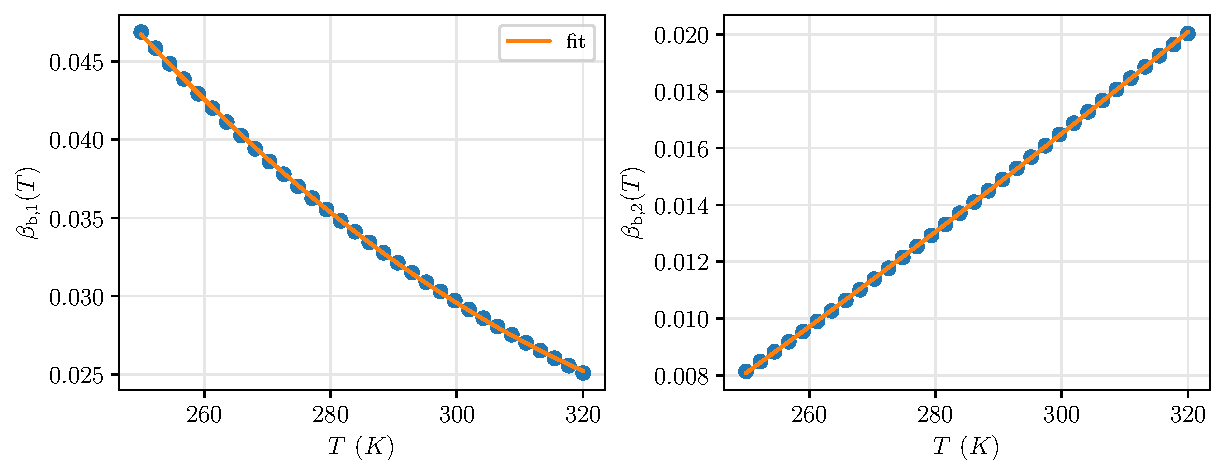
\includegraphics[width=0.9\textwidth]{radiation1}
    \caption{Band functions $\beta_\mathrm{b}(T)$ for the water vapor in the bands $150\pm 56~\mathrm{cm}^{-1}$ (left) and $1500\pm 40~\mathrm{cm}^{-1}$ (right). Symbols indicate values calculated with a numerical quadrature with a relative error of $10^{-8}$, and lines indicate the least squares parabolic fit.}\label{fig:radiation}
\end{figure}

\begin{table}
    \centering
    \footnotesize
    \renewcommand{\arraystretch}{1.2}
    \begin{tabular}{cccccc}
        \hline
        band & $\kappa_\mathrm{b}$ ($\mathrm{m}^2~\mathrm{kg}^{-1}$)& $a_0$ & $a_1$ ($\mathrm{K}^{-1}$) & $a_2$ ($\mathrm{K}^{-2}$) & rel. error (inf. norm) \\\hline
        $150\pm 56~\mathrm{cm}^{-1}$   & 130 & $2.6774\times 10^{-1}$ & $-1.3344\times 10^{-3}$ & $1.8017\times 10^{-6}$ & $0.5\%$ \\
        $1500\pm 40~\mathrm{cm}^{-1}$  & 8 & $-2.2993\times 10^{-2}$ & $8.7439\times 10^{-5}$ & $1.4744\times 10^{-7}$ & $0.7\%$ \\\hline
    \end{tabular}
    \caption{Coefficients of the least squares polynomial fit to the numerical quadrature of the band functions $\beta_\mathrm{b}(T)$ in the interval of temperatures $[250~\mathrm{K},320~\mathrm{K}]$}\label{tab:radiation}
\end{table}

\textbf{One model that is implemented in the code considers the water substance and a 3-band model. For the liquid, we consider a gray body. For the water vapor, we consider 2 bands: $150\pm 56~\mathrm{cm}^{-1}$ and $1500\pm 40~\mathrm{cm}^{-1}$ \citep{jeevanjee2023climate}. The third band is the rest of the frequency space outside of those 2 vapor bands, where the vapor absorption is zero but (I guess) not the dray air absorption? so far, I set it to zero.} The numerical calculation for the vapor bands is shown in Fig.~\ref{fig:radiation}. We consider a least squares polynomial fit of second order 
\begin{equation}
    \beta_\mathrm{b}(T)\approx a_0+a_1T+a_2T^2 \;.
\end{equation}
In this way, we mimic the polynomial fits to saturation pressure and heat capacities that are customary in numerical simulations. The coefficients for the 2 vapor bands are given in Table~\ref{tab:radiation}. The input parameters are $F_{\downarrow,z_\mathrm{max}}$, $\kappa_\mathrm{l}$, $\kappa_\mathrm{v,2}$, $\kappa_\mathrm{v,1}$ and the surface emissivity $\epsilon\in[0,1]$. 

\subsection{Microphysics}

Transport phenomena different from molecular transport, e.g., that due to particle sedimentation, can be considered as an additional source term $\mathrm{\bf Da}_\mathrm{T}\,\omega_\mathrm{T}\,\delta_{i\beta}$ in the right-hand side of one of the evolution equations, where $\mathrm{\bf Da}_\mathrm{T}$ is the corresponding nondimensional transport parameter and the transport function $\omega_\mathrm{T}^e(\zeta_j)$, to be provided, is normalized by the corresponding (dimensional) transport parameter.

For the transport function, see routine {\tt mappings/microphysics}.

